
\documentclass[12pt, a4paper]{report}
\usepackage{graphicx}
\usepackage{amsmath}
\usepackage{float}
\renewcommand{\baselinestretch}{1.2} 
\usepackage{ragged2e}
\usepackage{fancyvrb}
\usepackage{amssymb}
\usepackage[a4paper, total={6.5in, 8.5in}]{geometry}
\usepackage[utf8]{inputenc}



\title{\textbf{EE2703 : Applied Programming Lab \\ Assignment 4 \\ Fourier Approximation}} % Title
\author{Arun Krishna A M S \\ EE19B001} % Author name

\date{\today} % Date for the report

\begin{document}		
		
\maketitle % Insert the title, author and date
\justifying

\section*{Aim}
A Fourier series is a way of representing a periodic function as a (possibly infinite) sum of sine and cosine functions. In this assignment, we mainly focus on:
\begin{itemize}
  	\item Approximating functions $e^x$ and $cos(cos(x))$ in the range $[0,2\pi)$ by calculating fourier coefficients through
  	\begin{itemize}
      	\item Analysis Equation
      	\item Least Squares approach i.e., Curve fitting approach
  	\end{itemize}
  	\item Calculate the fourier series through the synthesis equation with coefficients obtained from both the methods
  	\item Study the error between the two approaches by plotting the coefficients obtained from the two methods
\end{itemize}

\section*{Introduction}

Consider a real valued periodic function that is integrable on an interval of length $2\pi$, which will be the period of the Fourier series. The \textbf{synthesis process} i.e., the actual Fourier series is given by:
 \begin{equation*}
F(x)=a_{0} + \sum_{n=1}^{N} \{a_{n}\cos(nx)+b_{n}\sin(nx)\}
 \end{equation*}

The weights: $a_0, a_1, a_2...,a_n...b_1,b_2...b_n..$ for the harmonics is determined by the \textbf{analysis equation}:
 \begin{align*}
a_{0}&=\frac{1}{2\pi}\int_{0}^{2\pi} f(x)dx\\
a_{n}&=\frac{1}{\pi}\int_{0}^{2\pi} f(x)\cos(nx)dx\\
b_{n}&=\frac{1}{\pi}\int_{0}^{2\pi} f(x)\sin(nx)dx\\
 \end{align*}

The existence of the fourier series alone doesn't determine the convergence or equality of $F(x)$ at all points.
At discontinuities

\begin{equation*}
F(c)=\frac{1}{2}(f(c^+)+f(c^-))
\end{equation*}

Fourier series doesn't converge at discontinuities, and at these discontinuities, Gibbs phenomenon takes place.

The assignment starts with defining the \texttt{exponential(x)} and \texttt{cosCos(x)} as

\begin{verbatim}
def exponential(x):
    return exp(x);
def cosCos(x):
    return cos(cos(x));
\end{verbatim} 

The expected fourier series is periodic with interval $2\pi$ when computed and plotted should look like

\begin{center}
	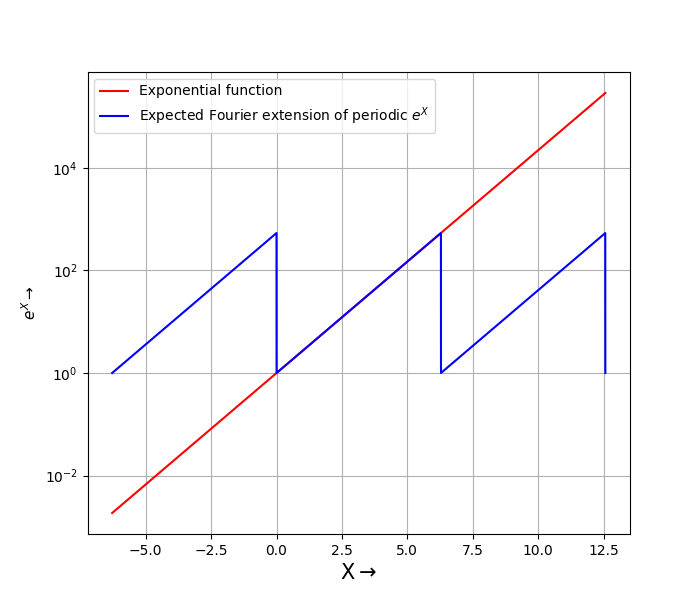
\includegraphics[scale=0.70]{Figure_1} 
	\caption{\\semilogY plot of $e^x$}
	\label{fig:rawdata}
\end{center}
\begin{center}
	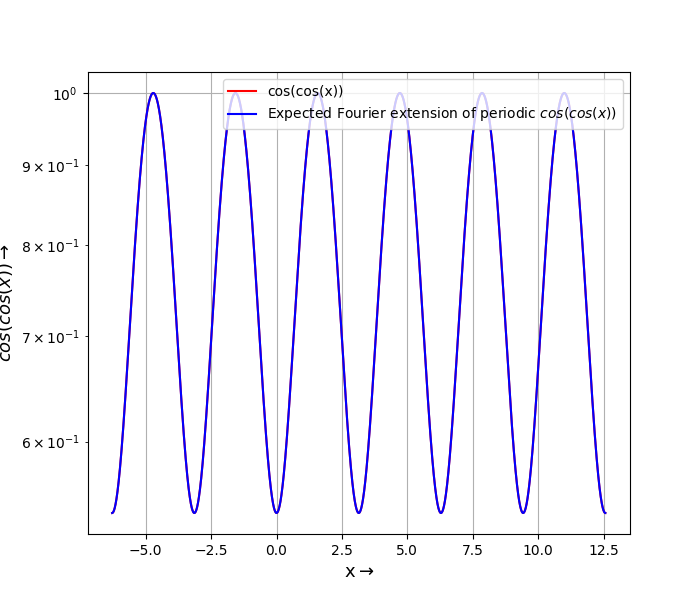
\includegraphics[scale=0.70]{Figure_2} 
	\caption{\\plot of $cos(cos(x))$}
	\label{fig:rawdata}
\end{center}

It can be observed that the function \textbf{$e^x$ is non-periodic while $cos(cos(x))$ is periodic} (Question 1) with periodicity $\pi$. Function $cos(cos(x))$ and its fourier series, overlaps with each other. It can be observed that fourier transform of $e^x$ repeats every $2\pi$ with discontinuities existing at the multiples of $2\pi$.

\section*{Generation of Fourier Coefficients}
The fourier coefficients is calculated by the analysis equation. In general, $N$ tends to $\infty$, but for all practical purposes, $N$ can be observed to be a large finite number. Here we consider only $N = 25$ which is sufficiently large. This may not be correct if the function is significantly made up of higher frequencies.

The functions $u(x,k)=f(x)\cos(kx)$ and $v(x,k)=f(x)\sin(kx)$ is generated by
\begin{verbatim}
func_dict = {'exponential(x)':exponential,'cosCos(x)': cosCos}
def u_Func(x,argument):
     k = argument[0];
     label = argument[1];
     func = func_dict[label];
     return func(x)*cos(k*x);

def v_Func(x,argument):
     k = argument[0];
     label = argument[1];
     func = func_dict[label];
     return func(x)*sin(k*x);
\end{verbatim} 

Functions $u(x,k)$ and $v(x,k)$ is then used in the analysis equation to determine the fourier coefficients. 
 \begin{align*}
a_{k}&=\frac{1}{\pi}\int_{0}^{2\pi} u(x,k)dx\\
b_{k}&=\frac{1}{\pi}\int_{0}^{2\pi} v(x,k)dx
 \end{align*}
 
 The integration is completed by the \texttt{scipy.integrate.quad}, with arguments for $u(x,k)$ and $v(x,k)$ is passed by creating the list \texttt{argument = [i,label]}

\begin{verbatim}
def functionCoefficient(label, numcoefficient):
     function = func_dict[label];
     cosCoefficient = np.zeros((numcoefficient+1)//2);
     sinCoefficient = np.zeros(numcoefficient//2);
     Coefficient = np.zeros(numcoefficient);
     
     cosCoefficient[0] = (SP.quad(function, 0, 2*pi)[0]) / (2*pi);
     Coefficient[0] = cosCoefficient[0];
     
     for i in range(1,cosCoefficient.size,1):
          argument = [i,label];
          cosCoefficient[i] = (SP.quad(u_Func,0,2*pi,args = argument)[0])/pi;
          Coefficient[2*i-1] = cosCoefficient[i];

     for i in range(1,sinCoefficient.size+1,1):
          argument = [i,label];
          sinCoefficient[i-1] = (SP.quad(v_Func,0,2*pi,args = argument)[0])/pi;
          Coefficient [2*i] = sinCoefficient[i-1];

     return Coefficient,cosCoefficient,sinCoefficient;
\end{verbatim} 
The fourier series coefficients is given by

\begin{equation*}
\texttt{Coefficient =}
\begin{pmatrix}
a_0\\
a_1\\
b_1\\
.\\
.\\
a_{25}\\
b_{25}\\
\end{pmatrix}
\hspace{0.5cm}
\texttt{cosCoefficient =}
\begin{pmatrix}
a_0\\
a_1\\
.\\
.\\
a_{25}\\
\end{pmatrix}
\hspace{0.5cm}
\texttt{sinCoefficient =}
\begin{pmatrix}
b_1\\
b_2\\
.\\
.\\
b_{25}\\
\end{pmatrix}
\end{equation*}

\section*{Visualization of Fourier Coefficients}
Fourier coefficients of $e^x$ are plotted below:
\begin{center}
	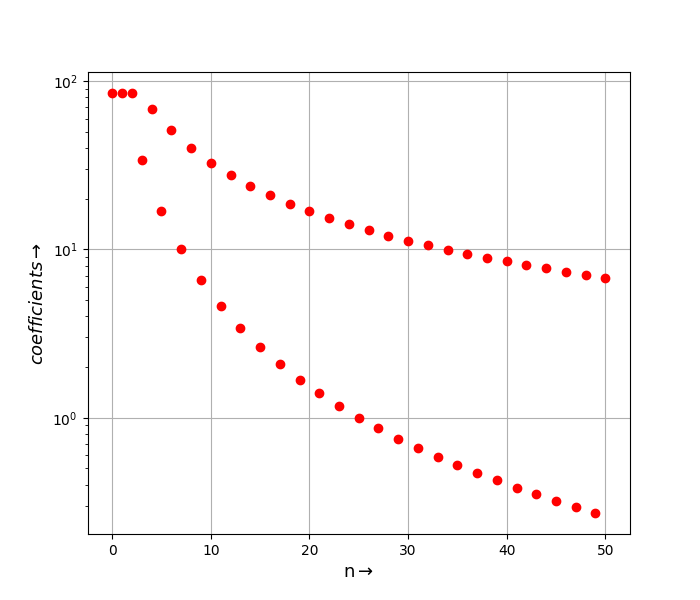
\includegraphics[scale=0.65]{Figure_3} 
	\caption{\\Fourier coefficients of $e^x$ (semilogY plot)}
	\label{fig:rawdata}
\end{center}
\begin{center}
	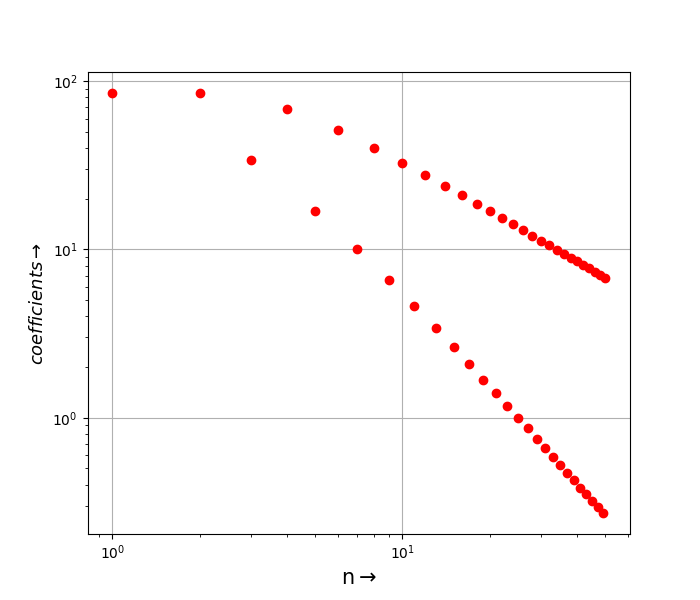
\includegraphics[scale=0.65]{Figure_4} 
	\caption{\\Fourier coefficients of $e^x$ (loglog plot)}
	\label{fig:rawdata}
\end{center}

 The coefficients of $e^x$ were found to be

 \begin{align*}
a_{k}&=\frac{1}{\pi}\int_{0}^{2\pi} e^xdx = \frac{e^{2\pi}-1}{\pi(1+k^2)}
\hspace{0.5cm}\implies a_k \propto \frac{1}{k^2} \hspace{0.5cm}\implies \log a_k \propto -2\log k\\
b_{k}&=\frac{1}{\pi}\int_{0}^{2\pi} e^xdx = \frac{k(1-e^{2\pi})}{\pi(1+k^2)} \hspace{0.5cm}\implies b_k \propto \frac{1}{k}\hspace{0.5cm}\implies \log b_k \propto -\log k
 \end{align*}

 Thus the \textbf{\texttt{loglog} plot for $e^x$ is found to be nearly linear} (Question 3c)
\\

It can be observed that $u(x) = cos(cos(x))cos(nx)$ and $v(x) = cos(cos(x))sin(nx)$ doesn't have closed form antiderivative. 

From \texttt{Figure 2}, we can intuitively say that the function $cos(cos(x))$ is periodic (with time period $\pi$), thus it is made up of low frequencies $\implies$ the \textbf{coefficients for higher frequencies for $cos(cos(x))$ decreases exponentially}. Whereas we observed earlier that the weight \textbf{for higher harmonics in $e^x$ is indirectly proportional to $k$ and $k^2$}. (Question 3b) 
\\

Fourier coefficients of $cos(cos(x))$ are plotted:
\begin{center}
	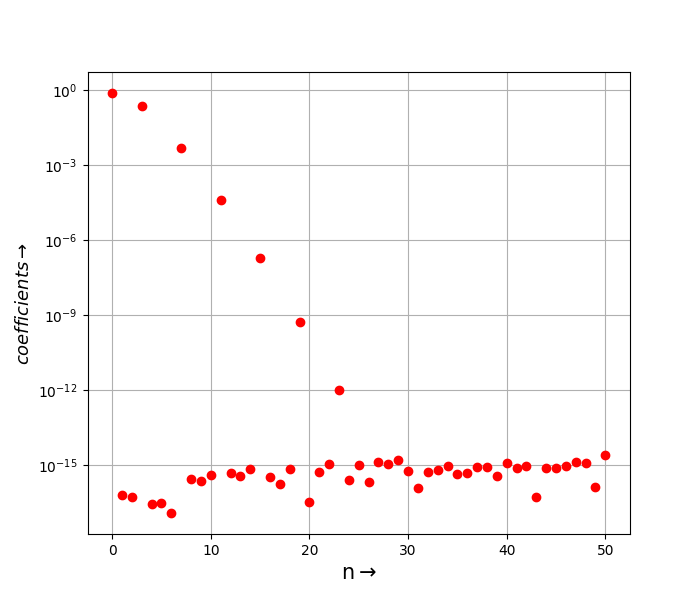
\includegraphics[scale=0.65]{Figure_5} 
	\caption{\\Fourier coefficients of $cos(cos(x))$ (semilogY plot)}
	\label{fig:rawdata}
\end{center}
\begin{center}
	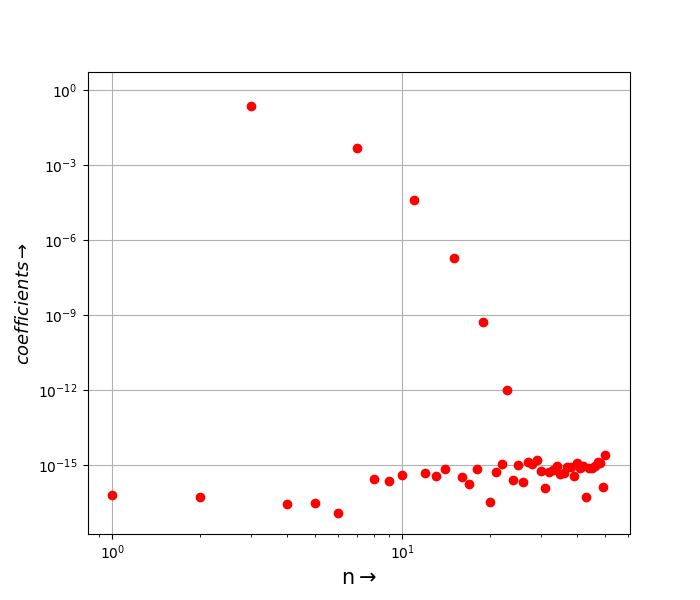
\includegraphics[scale=0.65]{Figure_6} 
	\caption{\\Fourier coefficients of $cos(cos(x))$ (loglog plot)}
	\label{fig:rawdata}
\end{center}

As expected, the coefficients for the second case decreases exponentially. This is shown in the \texttt{semilogY plot - figure 6} (Question 3b). 
\\

Note that $sin(x)$ function is odd, while $cos(x)$ function is even. Since the function $cos(cos(x))$ is even (i.e., $cos(cos(-x)) = cos(cos(x))$). This means that there are no odd sine components. Thus $b_n = 0$. Since the \texttt{quad} function computes integration numerically, values of $b_n$ may not be accurately be $0$. (Question 3a)

\section*{Fourier Coefficients by Linear Square Approach}

The first $51$ coefficients can also be approximately figured out by \textbf{Linear Square Approach}. Define a vector \texttt{X} going from $0$ to $2\pi$ in $400$ steps using \texttt{linspace}.
\begin{verbatim}
numData = 400;
X = np.linspace(0,2*pi,numData+1)[:-1];
\end{verbatim}

Evaluate the function $f(x)$ at those $x$ values and call it $b$. Now this function is to be approximated by the synthesis equation. So for each $x_i$ we want,
\begin{equation*}
a_{0} + \sum_{n=1}^{25} \{a_{n}\cos(nx_i)+b_{n}\sin(nx_i)\} \approx f(x_i)
\end{equation*}

Turning this into a matrix problem
\begin{equation*}
\begin{pmatrix}
1 & \cos x_1 & \sin x_1 & ... & \cos 25x_1 & \sin 25x_1 \\
1 & \cos x_2 & \sin x_2 & ... & \cos 25x_2 & \sin 25x_2 \\
... & ... & ... & ... & ... & ... \\
1 & \cos x_{400} & \sin x_{400} & ... & \cos 25x_{400} & \sin 25x_{400}
\end{pmatrix}
\begin{pmatrix}
a_0\\a_1\\b_1\\...\\a_{25}\\b_{25}
\end{pmatrix}
=
\begin{pmatrix}
f(x_1) \\ f(x_2) \\ ... \\ f(x_{400})
\end{pmatrix}
\end{equation*}

Let the matrix on the left side be $A$. We want to solve $Ac = b$ where $c$ are the fourier coefficients.
\begin{verbatim}
A = np.zeros((numData,numcoefficient));
A[:,0] = 1;
for i in range(1,(numcoefficient+1)//2):
     A[:,2*i-1] = cos(i*X);
     A[:,2*i] = sin(i*X);
\end{verbatim}

Using \texttt{scipy.linalg.lstsq} we solve this problem by executing
\begin{verbatim}
b = exponential(X);
C_Expo = scipy.linalg.lstsq(A,b)[0];

b = cosCos(X);
C_CosCos = scipy.linalg.lstsq(A,b)[0];
\end{verbatim}

This finds the “best fit” numbers that will satisfy the matrix equation at exactly the points we have evaluated $f(x_i)$. Plotting the obtained coefficients for the given functions. 

\begin{center}
	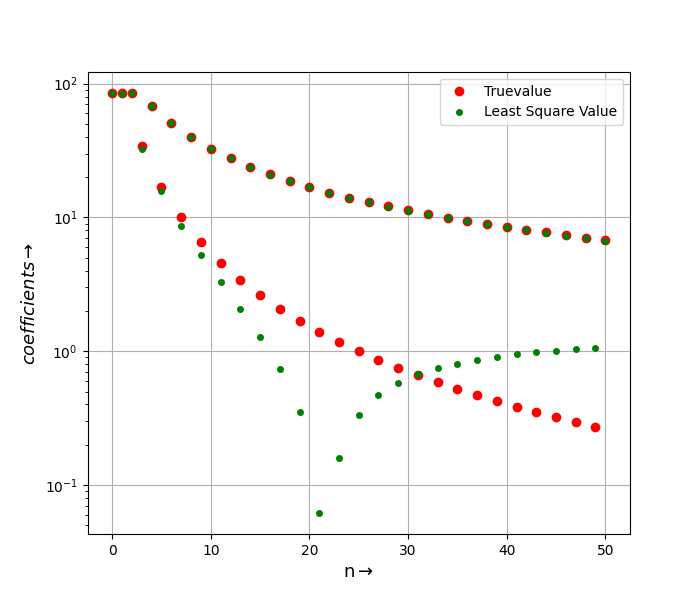
\includegraphics[scale=0.85]{Figure_7} 
	\caption{\\Fourier coefficients of $e^x$ (semilogY plot)}
	\label{fig:rawdata}
\end{center}
\begin{center}
	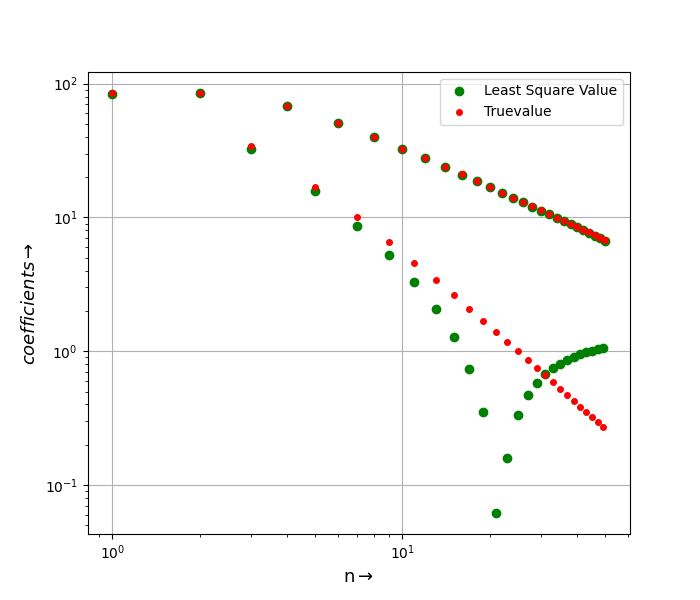
\includegraphics[scale=0.85]{Figure_8} 
	\caption{\\Fourier coefficients of $e^x$ (loglog plot)}
	\label{fig:rawdata}
\end{center}

\begin{verbatim}
errorMax_Exp = np.amax(np.abs(CoefficientExpo - C_Expo))
errorMax_CosCos = np.amax(np.abs(CoefficientCosCos - C_CosCos))
\end{verbatim}
\\

The maximum absolute error between the coefficients obtained from analysis equation and the coefficients obtained from least square method for the \textbf{function $e^x$ is
$1.3327308703354248$.} (Question 6)
\\

The maximum absolute error between the coefficients obtained from analysis equation and the coefficients obtained from least square method for the \textbf{function $cos(cos(x))$ is $2.682986310394032 \times 10^{-15}$. } (Question 6)
\\

\textbf{Our predictions for $e^x$ is worse compared to $cos(cos(x))$}.
The error deviation for $cos(cos(x))$ is plotted below.


\begin{center}
	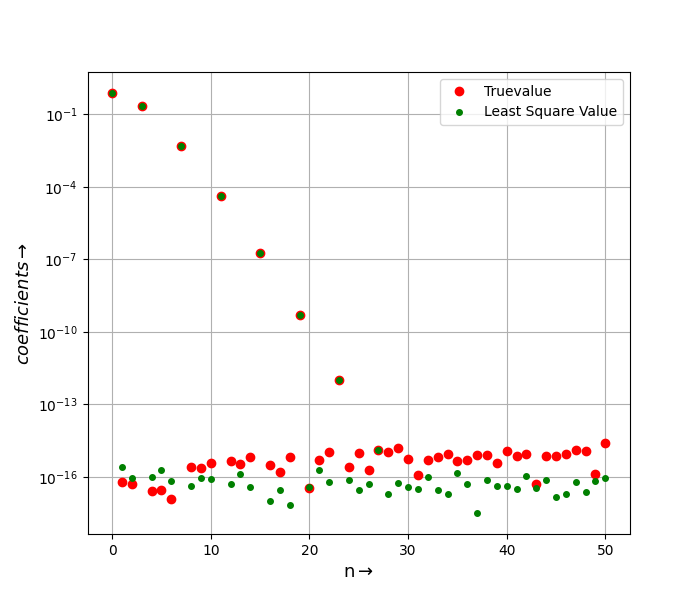
\includegraphics[scale=0.65]{Figure_9} 
	\caption{\\Fourier coefficients of $cos(cos(x))$ (semilogY plot)}
	\label{fig:rawdata}
\end{center}
\begin{center}
	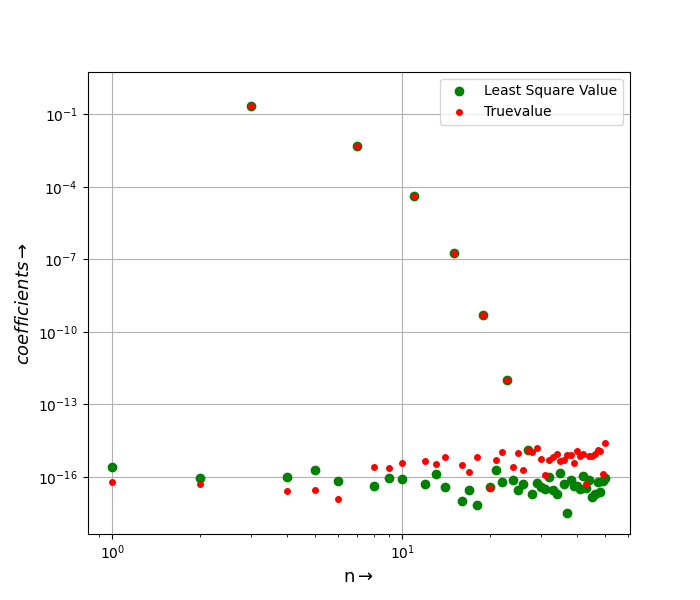
\includegraphics[scale=0.65]{Figure_10} 
	\caption{\\Fourier coefficients of $cos(cos(x))$ (loglog plot)}
	\label{fig:rawdata}
\end{center}

\section*{Function Approximation}

The matrix $V = Ac$ gives the approximate values at $(x_1,x_2,x_3...x_{400})$ where 
\begin{itemize}
  	\item $c$ column vector is calculated by the least square process
  	\item $c$ column vector is calculated by the analysis equation
\end{itemize}
and then plotted.

\begin{center}
	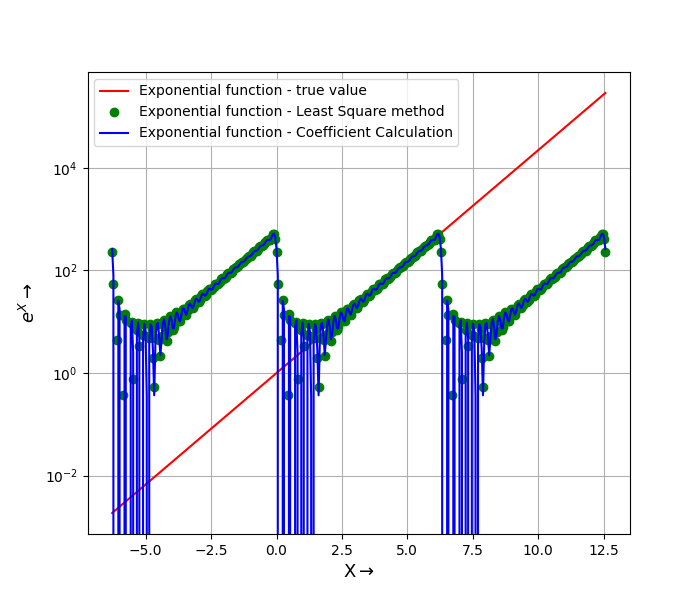
\includegraphics[scale=0.85]{Figure_11} 
	\caption{\\$e^x$ (semilogY plot)}
	\label{fig:rawdata}
\end{center}

The graph obtained by the analysis equation show rapid rise and fall at the discontinuities in the $e^x$ graph - \textbf{Gibbs Phenomenon}. The function $e^x$ has significant weight for higher frequencies, which is ignored in this calculation, resulting in great deviation.(Question 7) 

\begin{center}
	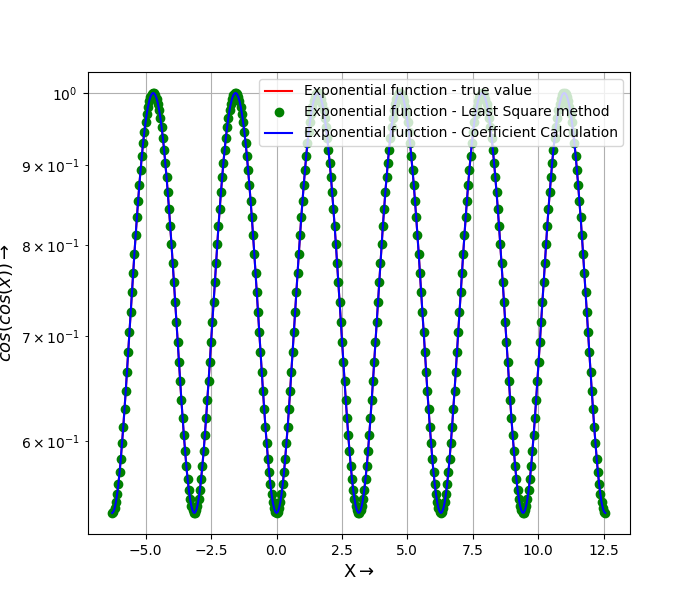
\includegraphics[scale=0.85]{Figure_12} 
	\caption{\\$cos(cos(x))$}
	\label{fig:rawdata}
\end{center}

The function $cos(cos(x))$ is predominantly made up of lower frequencies, thus the fourier series is very close to the actual function. Since the function doesn't have discontinuities, Gibbs Phenomenon is not observed.

Thus we can say that \textbf{fourier series of $cos(cos(x))$ is a much better approximate to the $cos(cos(x))$ compared to $e^x$} (Question 7)

\section*{Conclusion}
Fourier Coefficients of $cos(cos(x))$ and $e^x$ is calculated by both Analysis and Least Square method. We also observed that the presence of discontinuities and higher frequencies made the fourier series approximations for $e^x$ significantly diverge from its function compared to the function $cos(cos(x))$ 


\end{document}



 
